\section{问题一：典型风光场景下绿电直连指标分析}

\subsection{问题分析}

本问题要求在36吨/日初始产能下，假设电解槽与合成氨装置满负荷连续运行24小时，不计功率损耗，基于功率平衡原则计算园区典型日各项功率曲线和绿电直连指标。该问题本质上是一个代数计算问题，无需优化求解，关键在于正确建立功率平衡方程并准确计算各项指标。

\begin{figure}[H]
\centering
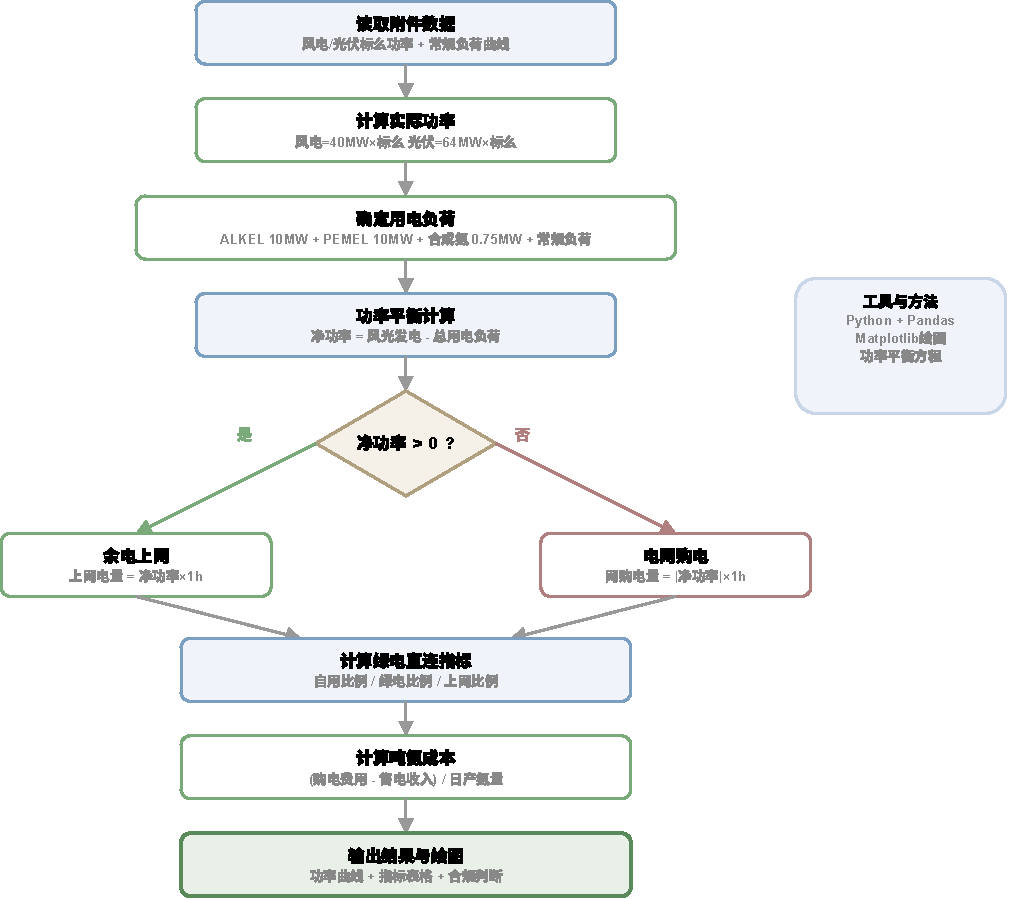
\includegraphics[width=0.85\textwidth,height=0.38\textheight,keepaspectratio]{../figures/fig_flow_q1.pdf}
\caption{问题一求解流程图}\label{fig:flow_q1}
\end{figure}

问题一的求解流程如图\ref{fig:flow_q1}所示，首先从附件数据中提取风电、光伏标幺功率曲线和常规电负荷标幺功率曲线，结合设备额定参数计算各时段实际功率，然后通过功率平衡方程确定购售电功率，最后计算电量指标和绿电直连三项指标。

\subsection{模型建立}

\subsubsection{设备参数确定}

在36吨/日产能下，各设备参数如下：碱性电解槽额定功率$P_{ALK}^{rated} = 10$ MW，产氢速率140 kg/h；质子交换膜电解槽额定功率$P_{PEM}^{rated} = 10$ MW，产氢速率160 kg/h；合成氨装置额定功率$P_{NH3}^{rated} = 0.75$ MW，产氨速率1.5 t/h。电氢氨装置总额定功率为：
\begin{equation}
P_{EHA}^{rated} = P_{ALK}^{rated} + P_{PEM}^{rated} + P_{NH3}^{rated} = 10 + 10 + 0.75 = 20.75 \text{ MW}
\end{equation}

\subsubsection{功率平衡方程}

每个时段$t$的功率平衡方程为：
\begin{equation}\label{eq:power_balance}
P_{wind}(t) + P_{pv}(t) + P_{buy}(t) = P_{EHA}^{rated} + P_{load}(t) + P_{sell}(t)
\end{equation}

其中$P_{buy}(t) \geq 0$，$P_{sell}(t) \geq 0$，且同一时段不能同时购售电。定义净功率为：
\begin{equation}
P_{net}(t) = P_{wind}(t) + P_{pv}(t) - P_{EHA}^{rated} - P_{load}(t)
\end{equation}

当$P_{net}(t) \geq 0$时，园区有余电上网，$P_{sell}(t) = P_{net}(t)$，$P_{buy}(t) = 0$；当$P_{net}(t) < 0$时，园区需从电网购电，$P_{buy}(t) = -P_{net}(t)$，$P_{sell}(t) = 0$。

\subsubsection{电量与指标计算}

日总用电量、新能源发电量、网购电量和上网电量分别为：
\begin{equation}
E_{total} = \sum_{t=1}^{24} [P_{EHA}^{rated} + P_{load}(t)] \cdot \Delta t, \quad E_{RE} = \sum_{t=1}^{24} [P_{wind}(t) + P_{pv}(t)] \cdot \Delta t
\end{equation}
\begin{equation}
E_{buy} = \sum_{t=1}^{24} P_{buy}(t) \cdot \Delta t, \quad E_{sell} = \sum_{t=1}^{24} P_{sell}(t) \cdot \Delta t
\end{equation}

绿电直连三项指标定义为：
\begin{equation}\label{eq:R1}
R_1 = \frac{E_{total} - E_{sell} - E_{buy}}{E_{RE}} \quad (\text{要求} > 60\%)
\end{equation}
\begin{equation}\label{eq:R2}
R_2 = \frac{E_{RE} - E_{sell}}{E_{total}} \quad (\text{要求} > 30\%)
\end{equation}
\begin{equation}\label{eq:R3}
R_3 = \frac{E_{sell}}{E_{RE}} \quad (\text{要求} < 20\%)
\end{equation}

\subsubsection{吨氨成本模型}

吨氨成本由风光度电成本、设备运维成本、购电成本和售电收入四部分构成：
\begin{equation}\label{eq:cost}
C_{ton} = \frac{C_{RE} + C_{OM} + C_{buy} - C_{sell}}{M_{NH3}}
\end{equation}

其中风光度电成本$C_{RE} = \sum_{t=1}^{24} [P_{wind}(t) \cdot c_{wind} + P_{pv}(t) \cdot c_{pv}] \cdot \Delta t \cdot 1000$，风电度电成本$c_{wind} = 0.15$元/kWh，光伏度电成本$c_{pv} = 0.12$元/kWh。设备运维成本$C_{OM} = (P_{ALK}^{rated} \cdot 0.1 + P_{PEM}^{rated} \cdot 0.15 + P_{NH3}^{rated} \cdot 0.002) \cdot 24 \cdot 1000$元。购电成本按分时电价计算，售电收入按上网电价$c_{sell} = 0.3779$元/kWh计算。

\subsection{求解结果}

\subsubsection{功率曲线分析}

将附件1的常规电负荷标幺功率曲线乘以峰值6 MW，附件2的风电、光伏标幺功率曲线分别乘以装机容量40 MW和64 MW，得到各时段实际功率值。典型日功率平衡曲线如图\ref{fig:q1_power_balance}所示。

\begin{figure}[H]
\centering
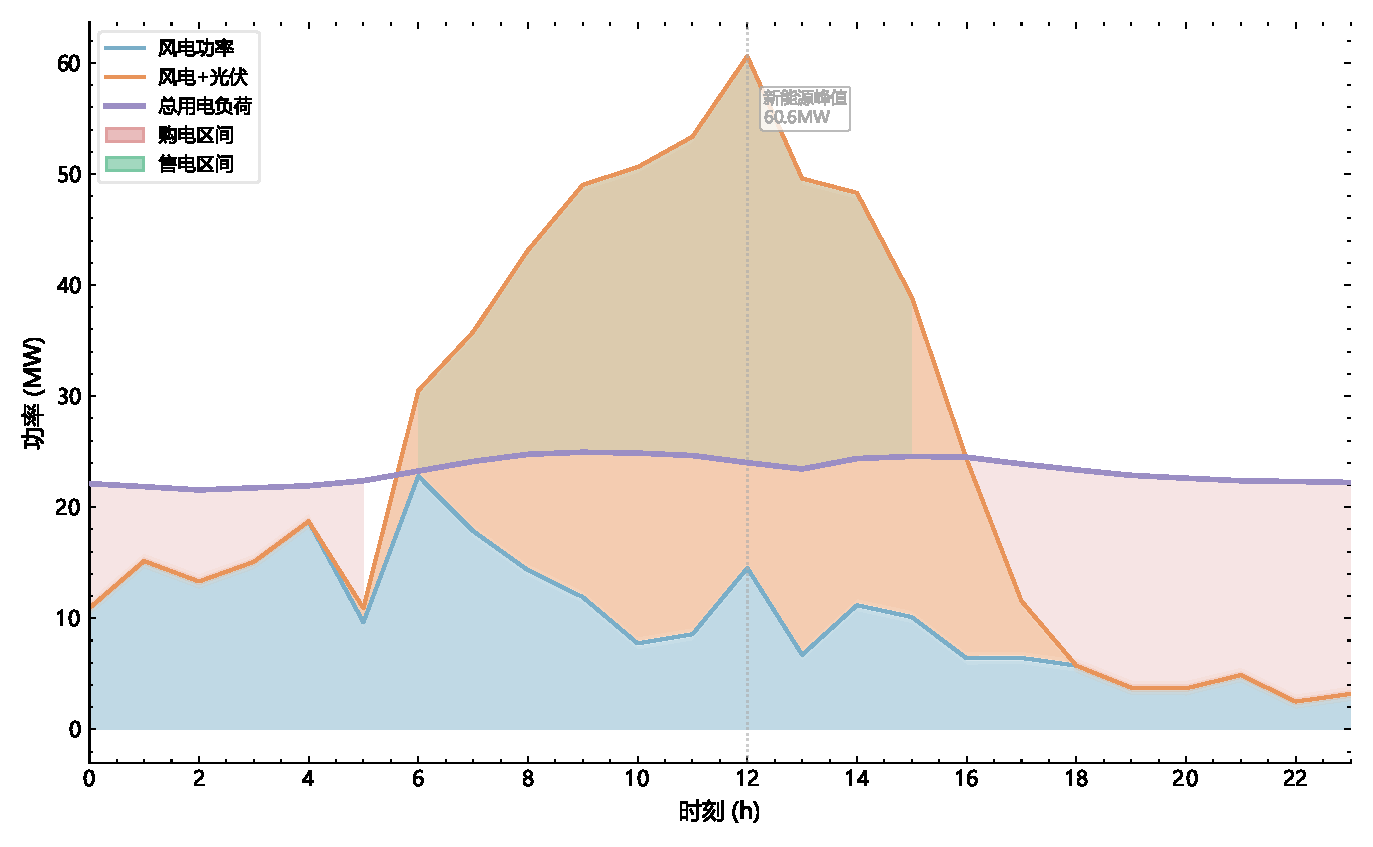
\includegraphics[width=0.85\textwidth,height=0.38\textheight,keepaspectratio]{../figures/fig_q1_power_balance.pdf}
\caption{典型日功率平衡曲线}\label{fig:q1_power_balance}
\end{figure}

从功率平衡曲线可以观察到明显的时段特征：白天时段（6:00--17:00）光伏出力强劲，风光总发电功率远超园区用电需求，产生大量余电上网，其中12:00时刻净余电功率达到峰值36.59 MW；夜间时段（18:00--次日5:00）光伏出力为零，仅靠风电难以满足园区20.75 MW的电氢氨装置功率加常规负荷，需要从电网大量购电，19:00时刻购电功率达到峰值19.12 MW。这种白天大量售电、夜间大量购电的"双向潮流"特征是导致绿电直连指标不达标的根本原因。

风光发电与负荷功率的详细对比如图\ref{fig:q1_power_detail}所示，进一步揭示了新能源出力与用电需求之间的时空错配特征。

\begin{figure}[H]
\centering
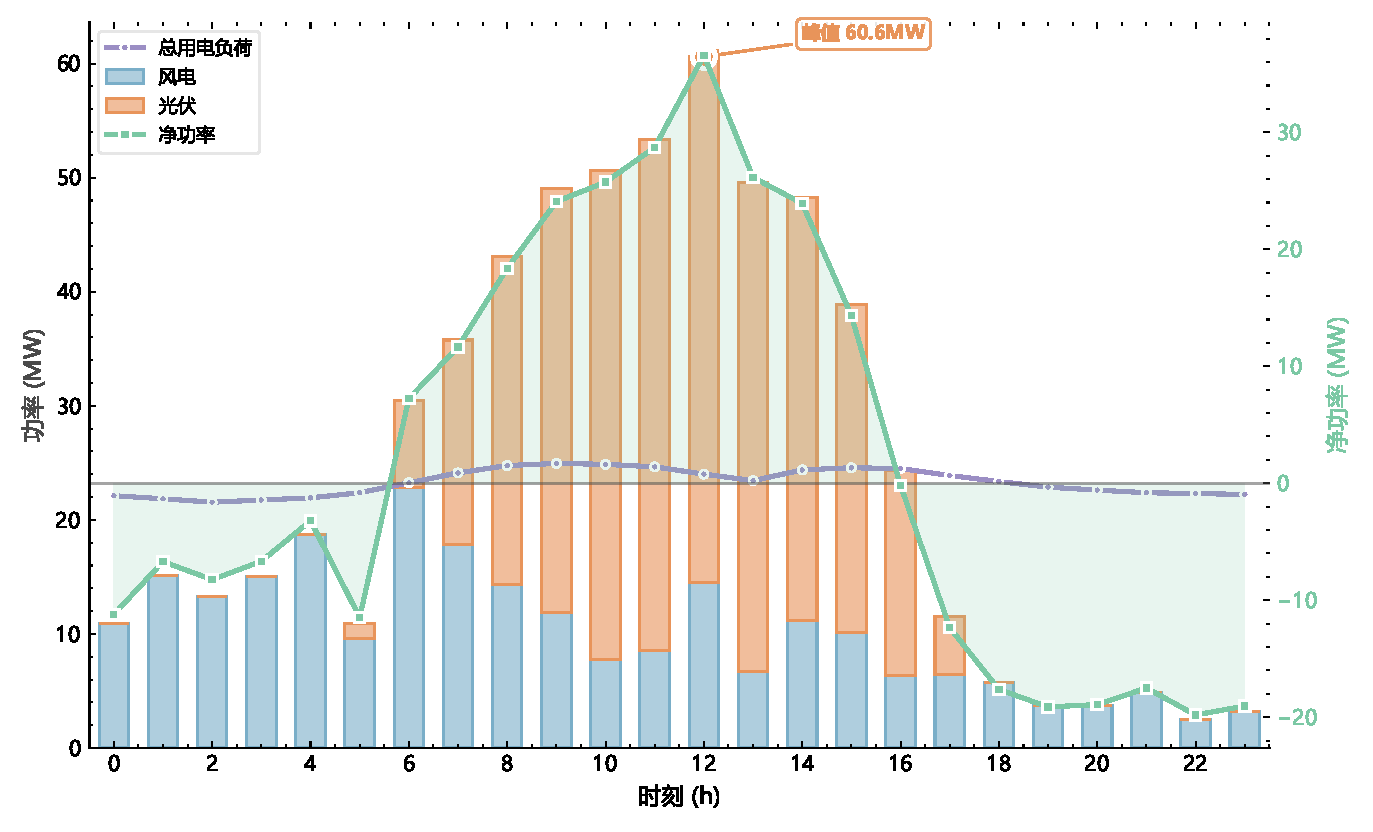
\includegraphics[width=0.85\textwidth,height=0.38\textheight,keepaspectratio]{../figures/fig_q1_power_detail.pdf}
\caption{风光发电与负荷功率对比及净功率变化}\label{fig:q1_power_detail}
\end{figure}

净功率曲线清晰地展示了园区在一天中经历的两个阶段：6:00--17:00为净发电阶段（净功率为正），18:00--次日5:00为净用电阶段（净功率为负）。光伏出力的集中性（峰值出现在12:00--13:00）与风电出力的波动性（凌晨和上午较强、傍晚较弱）共同决定了园区的购售电模式。

\subsubsection{电量指标与绿电指标}

\begin{table}[H]
\centering
\caption{问题一典型日各项电量指标及绿电指标汇总}
\begin{tabular}{lcc}
\toprule
指标 & 数值 & 是否达标 \\
\midrule
总用电量 (MWh) & 558.72 & — \\
新能源发电量 (MWh) & 603.45 & — \\
网购电量 (MWh) & 172.04 & — \\
上网电量 (MWh) & 216.77 & — \\
自发自用电量 (MWh) & 386.68 & — \\
\midrule
自发自用比 $R_1$ (>60\%) & 28.16\% & \textbf{否} \\
绿电比例 $R_2$ (>30\%) & 69.21\% & 是 \\
上网比例 $R_3$ (<20\%) & 35.92\% & \textbf{否} \\
吨氨成本 (元/吨) & 4322.34 & — \\
\bottomrule
\end{tabular}\label{tab:q1_indicators}
\end{table}

计算结果表明（表\ref{tab:q1_indicators}），在满负荷连续运行模式下，三项绿电直连指标中仅$R_2 = 69.21\%$满足大于30\%的要求，而$R_1 = 28.16\%$严重低于60\%的要求，$R_3 = 35.92\%$远超20\%的上限。

\subsection{指标不满足原因分析}

$R_1$不满足的直接原因在于其计算公式的分子$E_{total} - E_{sell} - E_{buy} = 558.72 - 216.77 - 172.04 = 169.91$ MWh，该值代表新能源自发自用电量中扣除了购售电的"净自用"部分。由于园区同时存在大量购电（172.04 MWh）和大量售电（216.77 MWh），分子被双向压缩，导致$R_1$仅为28.16\%。

$R_3$不满足的原因是白天光伏大量余电上网。光伏装机64 MW在正午时段出力可达44.8 MW，而园区总用电需求仅约25 MW，导致近20 MW的功率差额必须上网。全天上网电量216.77 MWh占新能源总发电量603.45 MWh的35.92\%，远超20\%上限。

从物理本质来看，问题的根源在于风光出力的时间分布与园区用电需求的时间分布存在严重错配：光伏出力集中在白天6小时内，而电氢氨装置需要24小时连续运行。这种时空错配在满负荷连续运行模式下无法通过调度手段缓解，必须引入负荷调节（问题二、三）或储能（问题四）来改善。
